\chapter{Planificación}
El proyecto se ha llevado a cabo durante un plazo de $8$ meses, con una carga de trabajo adecuada a la larga duración del proyecto, siempre teniendo en cuenta el tiempo de referencia con respecto a los créditos para intentar encajar la planificación en ese intervalo temporal.
Un trabajo de fin de grado consta de $12$ créditos ECTS, donde se estima que cada crédito debe valer unas $25$ horas de trabajo aproximadamente. Teniendo en cuenta estos datos, se calcula que la duración del TFG no debería ser superior a $300$ horas, teóricamente hablando. En la práctica se han visto sobre pasadas, no por mucho, para poder realizar un proyecto de calidad. Ha de tenerse en cuenta también que el alumno trabaja $25$ horas semanales y debe superar algunas asignaturas además de su proyecto final para terminar la carrera. Por lo tanto, el proyecto se planifica con una duración extendida en el tiempo, pero con una carga de trabajo semanal menos intensa.\\[6pt]
Se planifica una duración de $8$ meses aproximadamente, como ya se ha mencionado. Se utilizará un diagrama de Gantt~\cite{Clark1922} para describir la planificación del proyecto, de manera que se realizarán tareas en un orden cronológico, pero con superposición entre algunas. Varias tareas probablemente requerirán iteraciones posteriores, ya que es probable que se mejore y perfeccione el proyecto a lo largo de su ciclo de vida. Además hay otras tareas, como la investigación de metaheurísticas y la implementación de sus versiones binarias, que claramente se superponen, ya que tiene más sentido ir desarrollando cada una según se termina de estudiar para después comenzar con el siguiente algoritmo. \\[6pt]
Las fases del ciclo de vida son:
\begin{itemize}
      \item \textbf{Investigación inicial}
            Esto incluye investigar sobre conceptos básicos ya aprendidos, en forma de repaso sobre conceptos generales de aprendizaje automático, tipos de metaheurísticas, tipos de codificación, optimización de funciones, test estadísticos y conceptos básicos, código Python y librerías asociadas, instalación de estas a partir de un entorno virtual, configuración del entorno de trabajo e investigación sobre el problema de selección de características.

      \item \textbf{Diseño del software}: Planificación de la estructura general del código, uso de patrones de diseño que puedan ser de utilidad de cara a al mantenimiento del software a lo largo del desarrollo, concepto de modularización inicial del código (estructura del proyecto), uso de entornos virtuales.
      \item \textbf{Investigación metaheurísticas}: Realización de un estudio más exhaustivo acerca de las metaheurísticas a implementar y sus diferentes versiones binarias. Esto incluye un listado de $12$ metaheurísticas, cuya elección será justificada en posteriores secciones, siendo estas:
            \begin{itemize}
                  \item Firefly Algorithm
                  \item Whale Optimization Algorithm
                  \item Bat Swarm Optimizer
                  \item Grey Wolf Optimizer
                  \item Dragonfly Algorithm
                  \item Grasshopper Algorithm
                  \item Cuckoo Search
                  \item Differential Algorithm
                  \item Ant Colony Optimization
                  \item Artificial Bee Colony Optimization
                  \item Particle Swarm Optimization
                  \item Genetic Algorithm
            \end{itemize}
            De cada una de ellas se investigará su inspiración, funcionamiento, implementación y versiones binarias, normalmente asociadas al problema de selección de características.
      \item \textbf{Implementación del software}: Una vez claros los requisitos programáticos quedan establecidos, se implementará el software base. Esto incluye código en Python para la generación de gráficas, manejo de datasets en formato \textit{arff}, codificación de los algoritmos metaheurísticos en versión binaria, implementación de función objetivo (\textit{fitness}) y parametrización del programa para distintas pruebas.
      \item \textbf{Pruebas y refactorizado}: En esta etapa se llevarán a cabo pruebas exhaustivas para verificar la robustez y eficacia de los diferentes algoritmos implementados. Además, se considerará la refactorización del código si es necesario, con el fin de mejorar su estructura, claridad y mantenibilidad.
      \item \textbf{Análisis de resultados}: En esta fase se recopilarán datos de la ejecución de los algoritmos en sus diferentes versiones, así como entre ellos, utilizando los conjuntos de datos seleccionados para el proyecto. Esta recopilación de métricas permitirá una evaluación del rendimiento y la eficacia de cada algoritmo en comparación con los demás, así como su comportamiento en diferentes conjuntos de datos.
      \item \textbf{Documentación}: En esta etapa final se generará una documentación del proyecto que incluirá de forma general la descripción del problema, los objetivos, planificación, implementación, resultados y pruebas.
\end{itemize}

\begin{table}[H]
      \centering
      \begin{tabular}{c|c}
            Tarea                         & Duración (horas) \\ \hline
            Investigación inicial         & 20 \\
            Diseño del software           & 19 \\
            Investigación metaheurísticas & 85 \\
            Implementación del software   & 76 \\
            Pruebas y refactorizado       & 25 \\
            Análisis de resultados        & 30 \\
            Documentación                 & 91 \\ \hline
      \end{tabular}
      \caption{Tabla de duración de cada tarea}
\end{table}

\begin{figure}[H]
      \begin{center}
            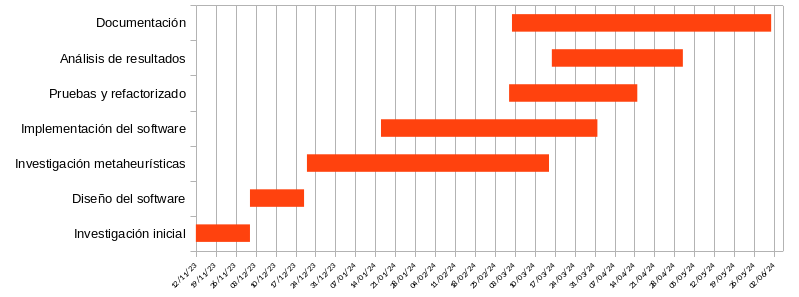
\includegraphics[width=1\textwidth]{imagenes/gantt-init.png}
      \end{center}
      \caption{Diagrama de Gantt inicial}
\end{figure}

La planificación inicial tiene en cuenta un curso ideal del ciclo de vida del proyecto, siendo las etapas más extensas la de creación del software e implementación de la documentación. En un diagrama de Gantt ideal las tareas serían excluyentes, pero como ya se ha mencionado, algunas tareas no son realistas si no se hacen paralelamente junto a otras.\\[6pt]
La planificación final del proyecto se ha modificado significativamente debido a una serie de contratiempos y obstáculos surgidos durante su desarrollo, así como la influencia de numerosos eventos externos que han afectado a su cronograma. En particular, se han experimentado retrasos y bloqueos que han incidido en la duración prevista del proyecto. Esto ha llevado a una re-evaluación de la estrategia de planificación original. Entre otras cosas, la implementación del software se ha visto alargada debido a numerosos parches.

\begin{figure}[H]
      \begin{center}
            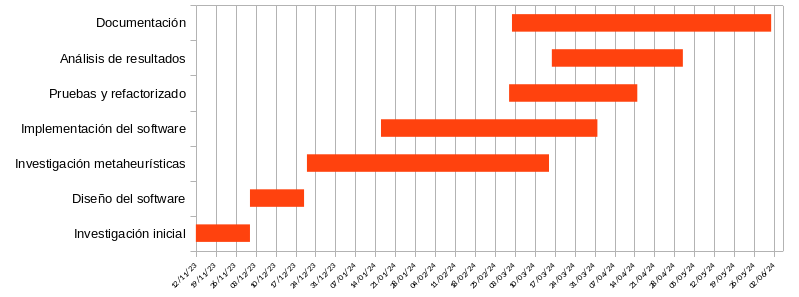
\includegraphics[width=1\textwidth]{imagenes/gantt-init.png}
      \end{center}
      \caption{Diagrama de Gantt final}
\end{figure}

El coste estimado del proyecto se divide en varios sub-costes:
\begin{itemize}
      \item \textbf{Sueldo}: Considerando un precio de proyecto que deba cubrir gastos y compensar, se estima un salario por investigador de $25$€/hora. El proyecto ha durado aproximadamente $8$ meses. Pese a ello, las horas trabajadas equivalen a un total de aproximadamente $400$ horas. Por tanto, el salario final total es de $10.000$€.
      \item \textbf{Ordenador portátil}: El estudiante consta con un portátil HP Pavilion Laptop 14-ec0xxx como herramienta principal de trabajo, con un precio de $1000$€. Ha sido usado durante unos $8$ meses aproximadamente. Si se tiene en cuenta que la vida media de un portátil es de aproximadamente $4-5$ años~\cite{woidasky_use_2021} entonces el costo del ordenador sería de $133.3$€.
      \item \textbf{Servidor} Para la experimentación del proyecto se ha hecho uso del servidor Hércules~\cite{citicugr}, por lo que el coste real ha sido de cero. Pese a ello, se estima cuanto costaría un servicio parecido en un servidor \textit{Cloud}. Se estima el precio por mes y total dada una estimación de los servicios de \textit{Google Cloud - Compute Engine}.
\end{itemize}
\begin{table}[H]
      \centering
      \begin{tabular}{|c|c|c|c|}
            \hline
            \textbf{Name}                            & \textbf{Quantity} & \textbf{Region} & \textbf{Service ID} \\
            \hline
            Compute optimized Core running in London & 150.0             & europe-west2    & 6F81-5844-456A      \\
            Compute optimized Ram running in London  & 600.0             & europe-west2    & 6F81-5844-456A      \\
            Storage PD Capacity in London            & 0.2               & europe-west2    & 6F81-5844-456A      \\
            \hline
      \end{tabular}
      \caption{Costos servidor Google Cloud - Part 1}
      \label{tab:server_costs_part1}
\end{table}
\begin{table}[H]
      \centering
      \begin{tabular}{|c|c|}
            \hline
            \textbf{SKU}   & \textbf{Total Price (USD)} \\
            \hline
            271A-7F2A-C5C5 & 6.56775                    \\
            0BD6-E233-D705 & 3.5202                     \\
            BF1A-6647-009D & 0.0096                     \\
            \hline
            Total Price:   & 10.09755                   \\
            \hline
      \end{tabular}
      \caption{Costos servidor Google Cloud - Part 2}
      \label{tab:server_costs_part2}
\end{table}
En la primera tabla, se detallan tres servicios distintos implementados en la región de Londres. Cada servicio se identifica por su nombre, cantidad (indicando la cantidad de recursos utilizados), región de implementación y un identificador único del servicio. Lo importante es que se ha calculado un servicio con $30$ vCPUs para paralelizar los trabajos.\\[6pt]

La segunda tabla complementa la primera proporcionando detalles adicionales sobre los servicios en términos de SKU (Stock Keeping Unit, una identificación única para un producto) y el precio total en dólares estadounidenses asociado con cada uno de ellos. El total, hecho el cambio de divisa a euros, es de $9.48$€ al mes, es decir, $75.84$€ en total (calculado para 8 meses).
Dado este desglose, se calcula el coste final del proyecto:
\begin{table}[h]
      \centering
      \begin{tabular}{|l|r|}
            \hline
            \textbf{Item}                    & \textbf{Costo (€)} \\ \hline
            Salario                          & 10.000             \\
            Ordenador portátil               & 133.3              \\
            Servidor CPU - GC Compute Engine & 75.84              \\
            \textbf{Total}                   & \textbf{10.209,14} \\ \hline
      \end{tabular}
      \caption{Costo estimado del proyecto}
      \label{tab:proyect_budget}
\end{table}